\section{Reverberation}
\gls{reverb} is an effect where the sound wave is reflected, and therefore the reflected waves haves another travelling time and amplitude to the listener than the initial sound directly from the source to the listener. This effect is a very frequently effect which happens each time sound can be reflected by walls, trees, table and other surfaces which reflect sound. The following \autoref{fig:reverb_reflect} shows the \gls{reverb} effect form one person, the sound source to another person, the listener \citep{reverb_expl}.

\begin{figure} [htbp]
 \centering
  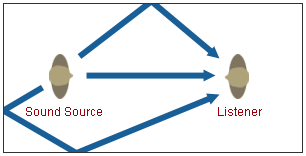
\includegraphics[width=0.6\textwidth]{reverb_reflect}
  \caption{The photo shows a echo in time domain}
  \label{fig:reverb_reflect}
\end{figure}

The received reflected sound is actually a series of very fast echo, which is merged together with all other reflected- and the direct sound, so the effect is notice as a single effect, although that may be more than 100 echos. 
\gls{reverb} make a complex echo which bring depth to the guitar, and make the sound from the guitar more natural \citep{reverb_natural}

A simple block diagram is shown at \autoref{fig:reverb_block}.

\begin{figure} [htbp]
 \centering
\begin{picture}(0,0)%
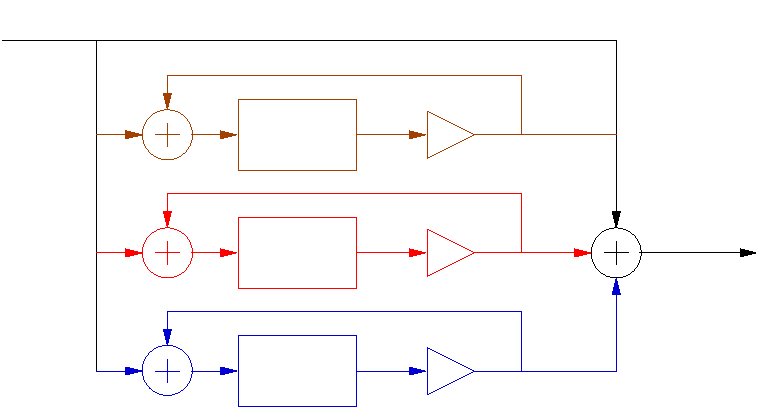
\includegraphics{reverb.pdf}%
\end{picture}%
\setlength{\unitlength}{4144sp}%
%
\begingroup\makeatletter\ifx\SetFigFont\undefined%
\gdef\SetFigFont#1#2#3#4#5{%
  \reset@font\fontsize{#1}{#2pt}%
  \fontfamily{#3}\fontseries{#4}\fontshape{#5}%
  \selectfont}%
\fi\endgroup%
\begin{picture}(5787,3102)(886,-1603)
\put(5896,-286){$Output$}%
\put(4321,704){$Gain$}%
\put(2791,1334){$Initial sound directly from the source$}%
\put(901,1334){$Input$}%
\put(2791,434){$Delay$}%
\put(2791,-466){$Delay$}%
\put(2791,-1366){$delay$}%
\put(4321,-241){$Gain$}%
\put(4321,-1141){$Gain$}%
\end{picture}%
  \caption{The photo shows a block diagram on a \gls{reverb} unit}
  \label{fig:reverb_block}
\end{figure}

The block diagram \autoref{fig:reverb_block} shows the direct sound way and only few delay block with individual gain, normally there will be many more delay lines. In the end, just before the Output line, all signals are added together.  